\documentclass[10pt]{article}
\usepackage[utf8]{inputenc}
\usepackage[includehead, headheight=10mm, margin=15mm ]{geometry}
\usepackage{amsmath}
\usepackage{amsthm}
\usepackage{amsfonts}
\usepackage{xcolor}
\usepackage{graphicx}
\usepackage{titling}
\usepackage{fancyhdr}
\usepackage{listings}

\title{APPM 4600 Homework 8}
\author{Edward Wawrzynek}
\date{25 October 2024}

\newcommand*{\dif}{\mathop{}\!\mathrm{d}}

\makeatletter
\def\@maketitle{%
  \newpage
  \null
  \vskip 1em%
  \begin{center}%
  \let \footnote \thanks
    {\LARGE \@title \par}%
    \vskip 1em%
    {\normalfont \@date}
  \end{center}%
  \par
  \vskip 1em}
\makeatother

\begin{document}

\pagestyle{fancy}
    \fancyhf{} % clear all header and footer fields
    \fancyhead[L]{\thetitle}
    \fancyhead[R]{\theauthor}

\makeatletter
\begin{center}
    {\Large \@title}
    \vskip 1mm
    {\normalfont \@date}
    \vskip 1em
\end{center}
\makeatother

The code used in this assignment is listed at the end.

\begin{enumerate}
    \item We wish to interpolate \begin{align*}
        f(x) = \frac{1}{1+x^2},
    \end{align*} which has derivative \begin{align*}
        f'(x) = -\frac{2x}{(1+x^2)^2}.
    \end{align*} We perform Lagrange, Hermite, and cubic interpolations of \(f\) over \([-5, 5]\) with equispaced nodes. The results are plotted below for \(N=5,10,15,20\) nodes.

    Notice that Lagrange and Hermite interpolation display the Runge phenomenon for large \(N\), while the cubic interpolations do not. This is expected---the cubic interpolations are piecewise between points, so they don't suffer unbounded growth as \(N\) increases. In general, the cubic interpolations match the function best, with natural splines having smaller error as \(N\) grows.

    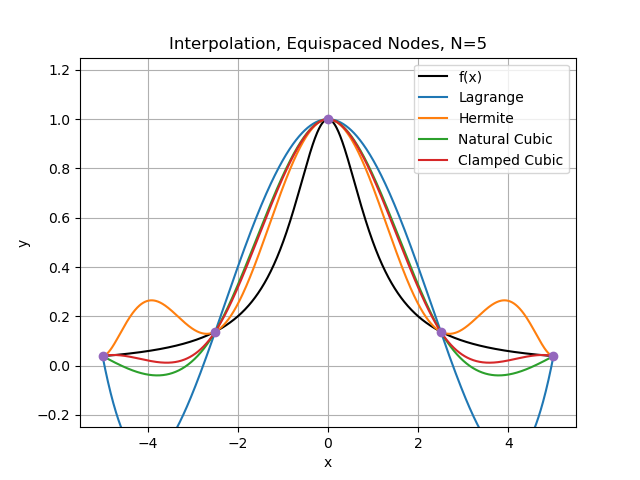
\includegraphics[width=0.49\textwidth]{equi_N5_interp.png}
    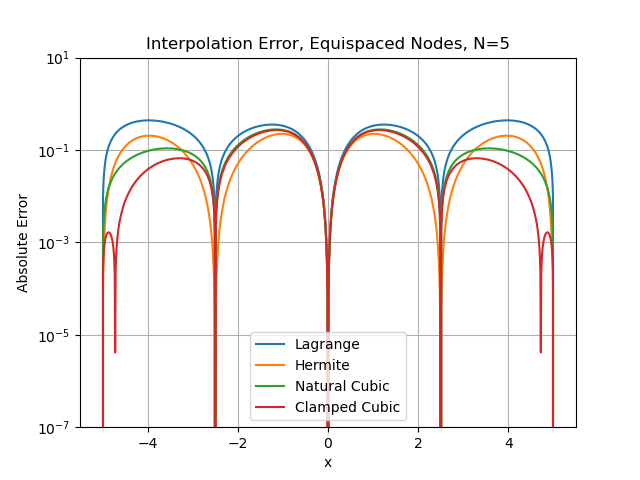
\includegraphics[width=0.49\textwidth]{equi_N5_error.png}
    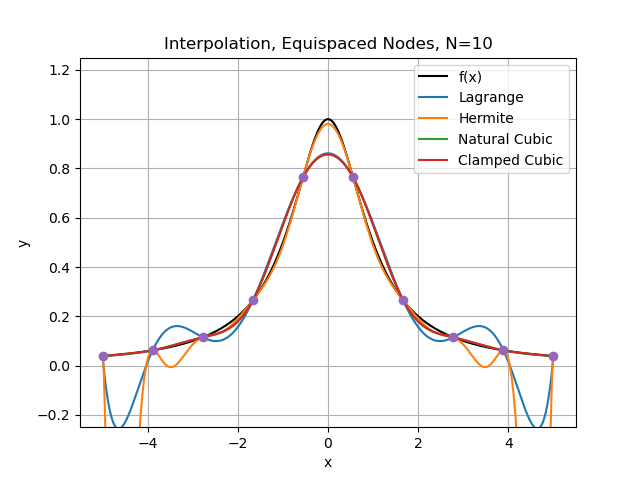
\includegraphics[width=0.49\textwidth]{equi_N10_interp.png}
    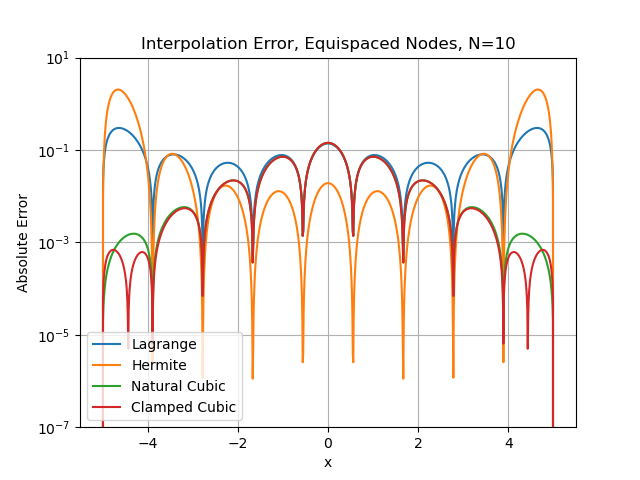
\includegraphics[width=0.49\textwidth]{equi_N10_error.png}
    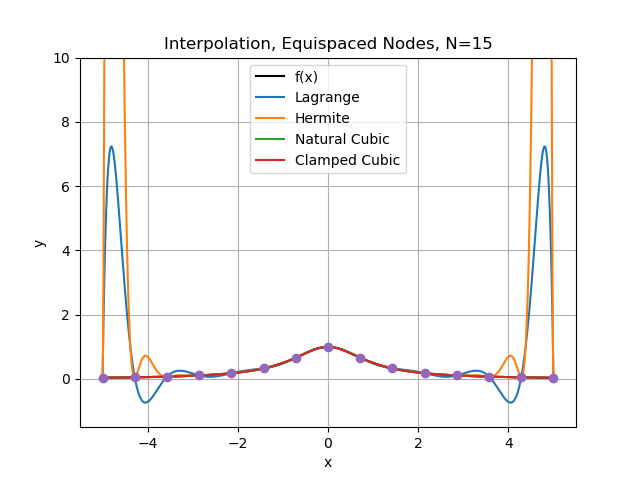
\includegraphics[width=0.49\textwidth]{equi_N15_interp.png}
    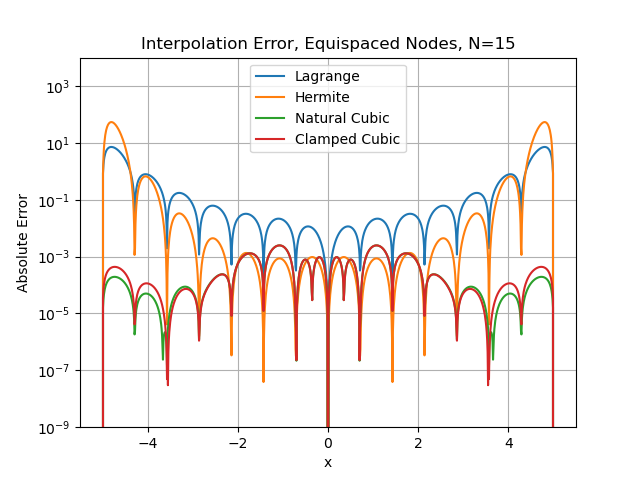
\includegraphics[width=0.49\textwidth]{equi_N15_error.png}
    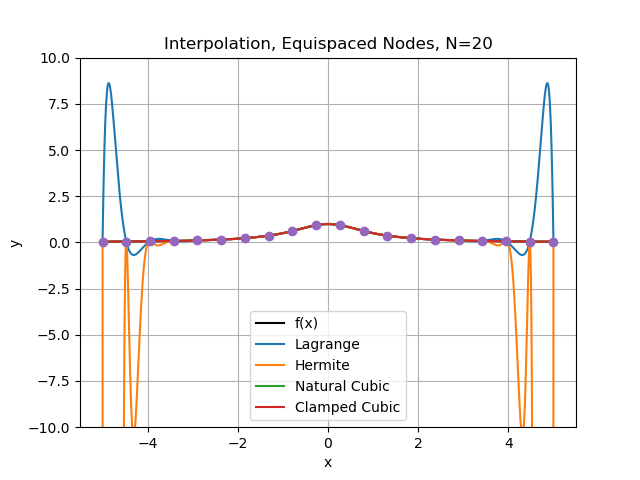
\includegraphics[width=0.49\textwidth]{equi_N20_interp.png}
    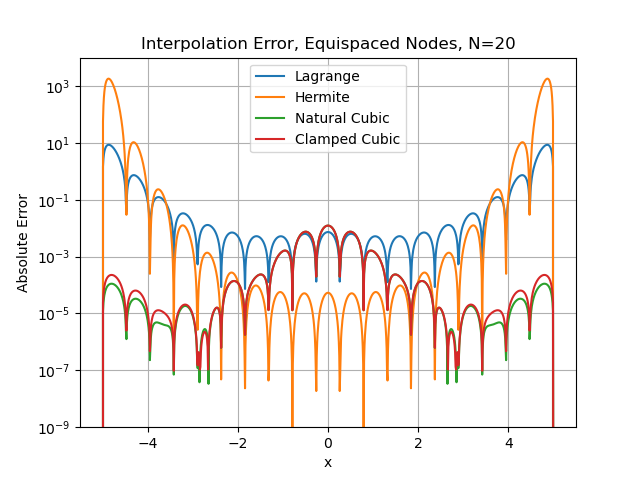
\includegraphics[width=0.49\textwidth]{equi_N20_error.png}

    \newpage
    \item We construct the Chebychev nodes of the second kind, \begin{align*}
        x_i = \cos  \left( \frac{i}{N-1}\pi \right),\;n=0,1,\dots,N-1.
    \end{align*} We perform the same interpolation as in the previous question over these nodes, yielding results plotted below.

    Notice that the Chebychev nodes are effective in eliminating the Runge phenomenon in the Lagrange and Hermite interpolations. All the interpolations are able to get reasonably close to the function. The cubic interpolations perform worse near \(x=0\) than they did with equispaced nodes, which is expected---the relative lack of nodes in this area will hurt their accuracy. In general, the Hermite interpolation has lowest error as \(N\) grows, although the cubic interpolations still perform better near the edges.

    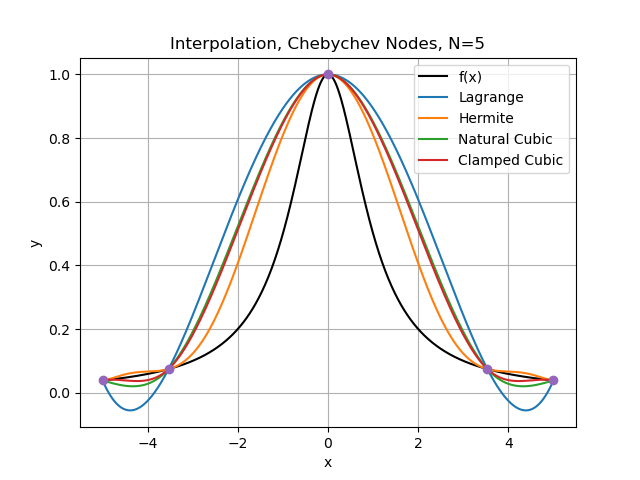
\includegraphics[width=0.49\textwidth]{cheb_N5_interp.png}
    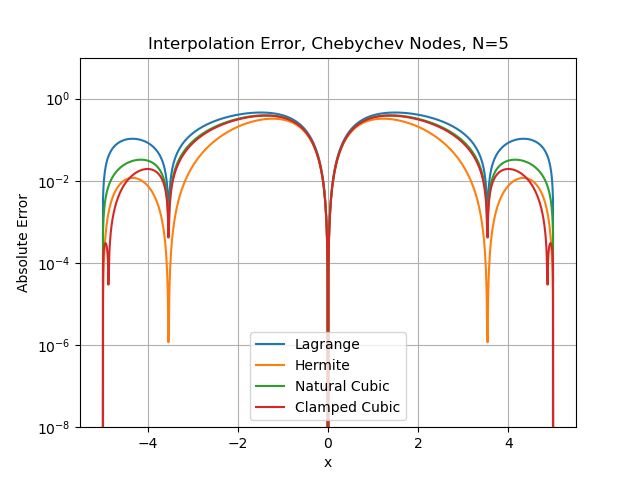
\includegraphics[width=0.49\textwidth]{cheb_N5_error.png}
    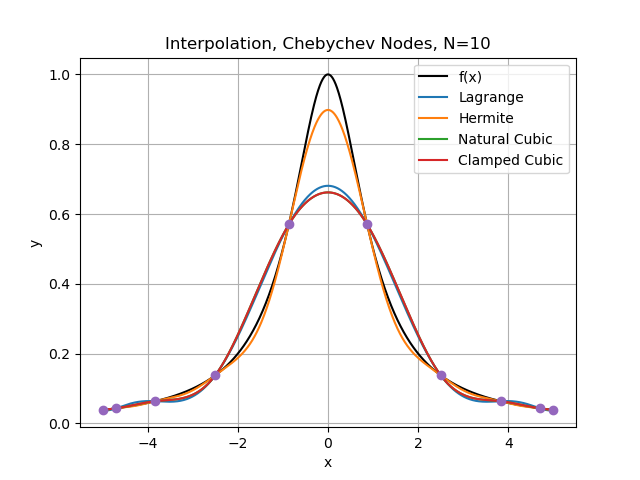
\includegraphics[width=0.49\textwidth]{cheb_N10_interp.png}
    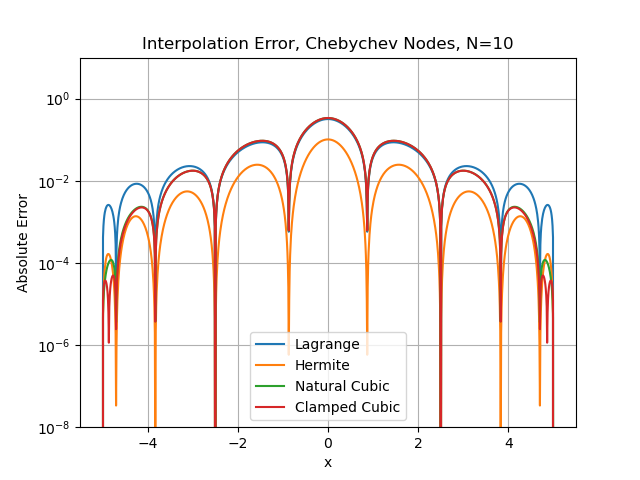
\includegraphics[width=0.49\textwidth]{cheb_N10_error.png}
    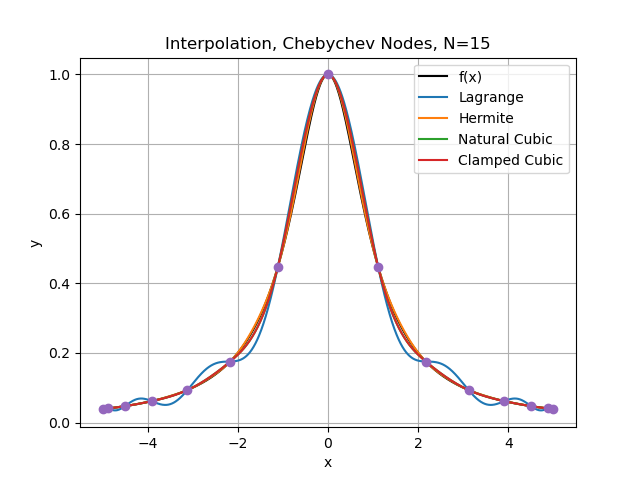
\includegraphics[width=0.49\textwidth]{cheb_N15_interp.png}
    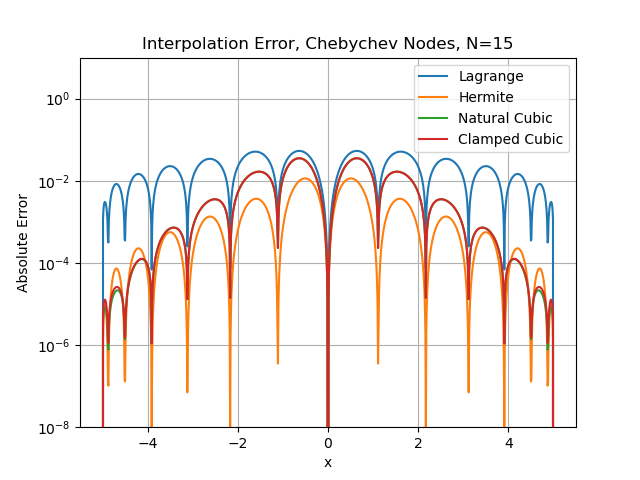
\includegraphics[width=0.49\textwidth]{cheb_N15_error.png}
    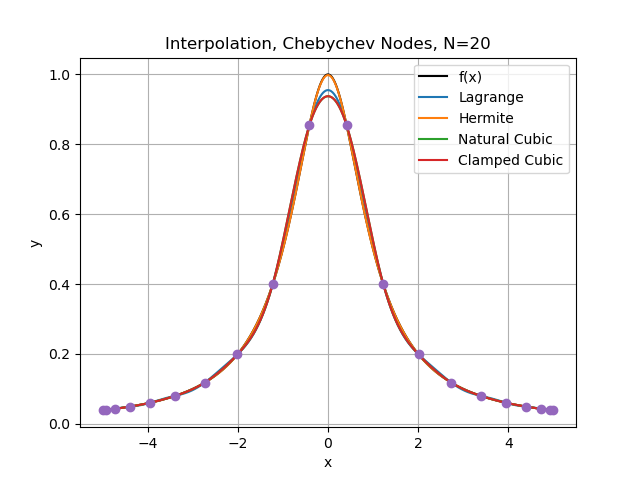
\includegraphics[width=0.49\textwidth]{cheb_N20_interp.png}
    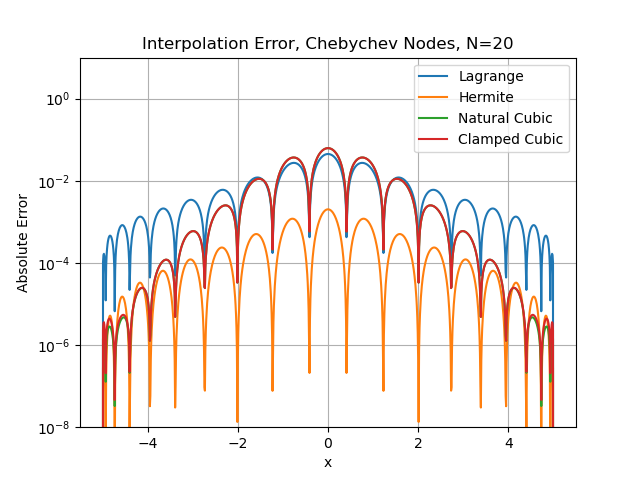
\includegraphics[width=0.49\textwidth]{cheb_N20_error.png}

    \newpage
    \item For a periodic spline, we want the periodic boundary conditions \begin{align}
        S_0(x_0) &= S_{n-1}(x_n)\\ S_0'(x_0) &= S_{n-1}'(x_n)\\S_0''(x_0) &= S_{n-1}''(x_n).
    \end{align}

    The condition (1) is enforced by periodicity of the function being interpolated and the fact that we force the spline to match the function at the endpoints. The third condition (3) gives \begin{align*}
        0 &= S_0''(x_0) - S_{n-1}''(x_n) \\
          &= M_0 - M_n,
    \end{align*} that is, \(M_0 = M_n\). The second condition (2) gives \begin{align}
      0 &= S_0'(x_0) - S_{n-1}'(x_n) \nonumber \\
        &= -\frac{h_0^2M_0}{2h_0} + \frac{f(x_1) - f(x_0)}{h_0} - \frac{M_1 - M_0}{6}h_0 - \left( -\frac{h_{n-1}^2M_n}{2h_{n-1}} + \frac{f(x_n) - f(x_{n-1})}{h_{n-1}} - \frac{M_n - M_{n-1}}{6}h_{n-1} \right) \label{eq:period_mess}.
    \end{align} We have from periodicity that \(f(x_0) = f(x_n)\), so \eqref{eq:period_mess} becomes \begin{align*}
        0 &= -\frac{h_0M_0}{2} + \frac{f(x_1) - f(x_0)}{h_0} - \frac{M_1 - M_0}{6}h_0 + \frac{h_{n-1}M_0}{2} - \frac{f(x_0) - f(x_{n-1})}{h_{n-1}} + \frac{M_0 - M_{n-1}}{6}h_{n-1},
    \end{align*} which we can rearrange to yield \begin{align*}
        \frac{f(x_{n-1})}{h_{n-1}} + \frac{f(x_1)}{h_0} - f(x_0) \left( \frac{1}{h_0} + \frac{1}{h_{n-1}} \right) &= \left(\frac{h_0}{2} - \frac{h_0}{6} - \frac{h_{n-1}}{2} - \frac{h_{n-1}}{6}\right)M_0 + \left( \frac{h_0}{6} \right)M_1 + \left( \frac{h_{n-1}}{6} \right)M_{n-1}. \\
    \end{align*}
    Notice that this has added an $M_{n-1}$ term into relationship we found previously for the natural splines. The matrix A becomes \begin{align*}
        A = \begin{bmatrix}
            \frac{h_0}{3} & \frac{h_0}{6} & 0 & \dots & & \frac{h_{n-1}}{6} \\
            \frac{h_0}{6} & \frac{h_1+h_0}{3} & \frac{h_1}{6} & 0 & \dots & 0 \\
            \dots & \\\
            0 & \dots  & &\frac{h_{n-2}}{6} & \frac{h_{n-1} + h_{n-2}}3 & \frac{h_{n-1}}{6} \\\
            \frac{h_0}{6} & \dots  & 0 & 0 * \frac{h_{n-1}}{6} & \frac{h_{n-1}}{3}
        \end{bmatrix}.
    \end{align*} 


\end{enumerate}
\newpage
{\small \lstinputlisting[language=Python]{hw8.py}}

\end{document}
